\subsection{Experiment 10} \label{sec:exp10}

The GANmix model is made possible by the use of a pre-trained \ac{VAE}. In other words, the GANmix generator tries to generate encodings that are similar to those produced by the \ac{VAE}. The \ac{VAE} uses \acp{CNN}, which explains why the \ac{GAN} models also use encodings.

However, what the GANmix model actually produces are embeddings that have no significant spatial relationship.

This experiment builds on the notion that fully connected neural networks may provide better results.

To achieve this, the models were modified so that the generator has a connection (fully connected linear layer) from the input to the hidden layer, and another connection from the hidden layer to the output (the embeddings). The discriminator follows a similar model architecture.

Other configuration aspects such as loss function, regularization techniques, data set, optimizer, and hardware configuration remained unchanged.

The experiment incurred a total loss of $6.425$, with $6-987$ pertaining to the generator loss and $-0.562$ to the discriminator loss.

For a visual representation of the results, which includes the loss, the histogram of the generated embeddings and the final spectrogram generated in this experiment, please see Figure~\ref{fig:exp10_results}.

The data shows a curious pattern: the discriminator loss steadily decreases as the generator loss continuously increases. This trend could be due to insufficient epochs, problems with the optimizer, or the lack of a suitable scheduler. However, based on previous experiments, the criterion seems unlikely to be the primary cause.

\begin{figure}[!ht]
    \centering
    \begin{subfigure}{0.3\textwidth}
        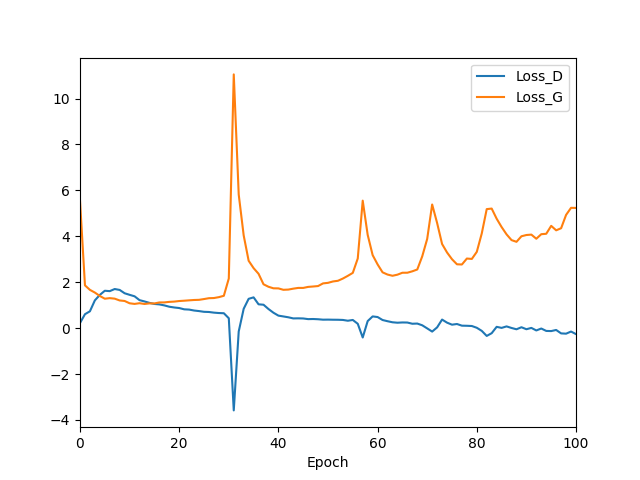
\includegraphics[width=\textwidth]{figures/4.5-results/exp10_loss.png}
        \caption{Evolving losses throughout the training process for Experiment 10.}
        \label{fig:exp10_loss}
    \end{subfigure}
    \begin{subfigure}{0.3\textwidth}
        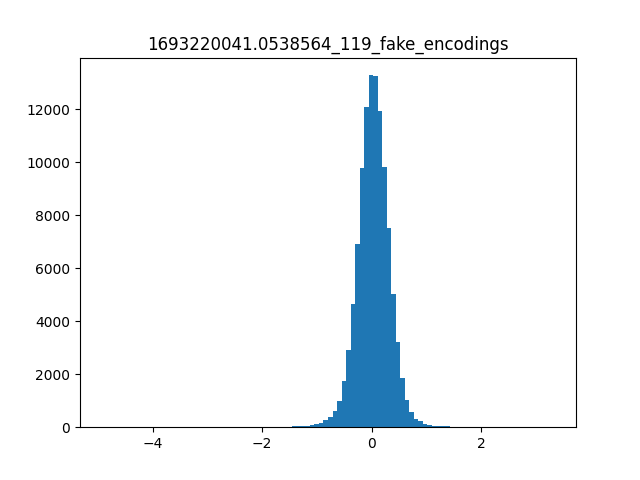
\includegraphics[width=\textwidth]{figures/4.5-results/exp10_hist.png}
        \caption{Histogram of the generated embeddings for Experiment 10.}
        \label{fig:exp10_hist}
    \end{subfigure}
    \begin{subfigure}{0.3\textwidth}
        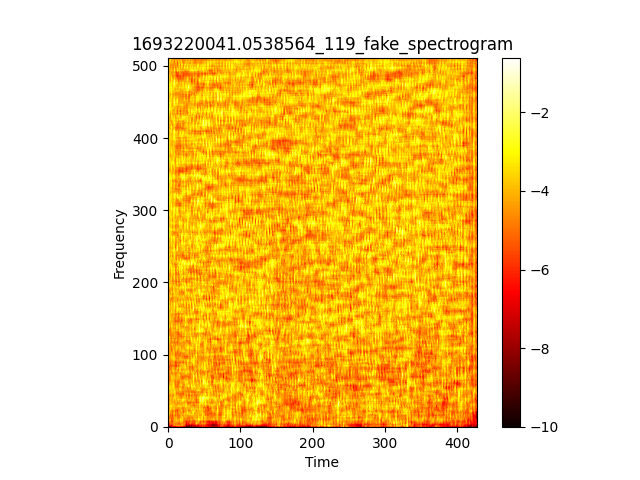
\includegraphics[width=\textwidth]{figures/4.5-results/exp10_spectrogram.png}
        \caption{Spectrogram generated in Experiment 10.}
        \label{fig:exp10_spectrogram}
    \end{subfigure}
    \caption{Results of Experiment 10.}
    \label{fig:exp10_results}
\end{figure}